\chapter{Introduction (English)}
\label{chap:intro-en}

\margintoc

This thesis belongs to the domain of \kl[dependent type]{type theory}, itself
at the crossroads between computer science and mathematical logics.
One of its goals is to give theoretical and practical foundations
for software tools helping humans in constructing and verifying proofs –
in the mathematical sense.
Such tools are called \kl{proof assistants}, and in this thesis one of them, on
which my work was mainly focused, is central: \kl{Coq}.

To replace this work in its larger context, this introduction begins with a very
short history of mathematical logics (\cref{sec:logic-history}), which exposes the
main problematics of the field. Follows a presentation of the links between logics and
computer science, through \kl{proof assistants} (\cref{sec:proof-assistants}).
Next, \cref{sec:intro-coq-en} focuses more closely on the research ideas and problematics
I worked on.
Finally, \cref{sec:this-thesis} summarizes the contributions appearing in the rest of
this thesis.

\section{A very short history of logics}
\label{sec:logic-history}

\subsection{Syllogisms}

The main question that logics looks to answer is that of finding criteria in order to determine
if a reasoning is valid. In Western tradition, this problematic can be traced back to the
Antiquity, and particularly to Aristotle, with his \textit{Organon}.
The main contribution of this work is to introduce the notion of syllogism.
These are simple fragments of reasoning, the validity of which stems from the
fixed structure they follow, rather than a specific content.%
\sidenote{The most well-known is probably the \textit{Barbara} syllogism, and example
of which is: \emph{all humans are mortals; Socrates is human; so Socrates is mortal.}}
If complex reasoning is built by assembling such syllogisms, it must necessarily be valid as
a whole, since every assembled fragment is. There are here two important ideas.

The first is that reasoning can be valid or not depending only on its structure,
independently of its content. Indeed, the whole focus of logics as a discipline from that
point on will concentrate on this structure which underlies reasoning.
It can be syllogisms, but many other systems. We will come across a certain number of them
in this thesis!

The second is that of a construction from elementary components. Starting from a set of rules
one has identified as valid \textit{a priori}, we have a means to ensure the validity
of potentially very complex reasoning. In order to do so, it suffices to verify that these
can be decomposed into the base components.

At that time already, logics was conceived as a means towards communication.
The aim was of course to check one’s own reasoning, but also to be able to exchange
it, by fixing a logical formal system%
\sidenote{Structural rules reasoning should obey, as those of syllogisms.}.
A person wanting their conclusion to be accepted by others just has to express their
reasoning in a perfectly precise way in the framework of such a formal system.

The main challenge of logics is thus to construct such a formal system, adapted to a specific
field of reasoning. In the case we are interested in, this of mathematical logics, this
enables us to give a precise meaning to what constitutes a valid mathematical proof.


\subsection{The beginning of mathematical logics: towards a formal foundation}

Following Aristotle, mathematicians seized logics in order to build a formal system
able to serve as a rigorous foundation for mathematics.
Even though the links between logics and mathematics go back to Greek Antiquity,
important advances happened during the 19\textsuperscript{th} century, on two main aspects.

The first consisted in freeing mathematical logics from natural languages%
\sidenote{By opposition with the formal languages which appear in mathematics,
  computer science, etc.},
unsuited to a formal description of deduction, and to instead design a new form of language
specific that could serve as a basis for mathematical reasoning.
An important step here is \citeauthor{Begriffsschrift}'s
\citetitle{Begriffsschrift}~\sidecite{Begriffsschrift}, which, for the first time,
gives a formal language rich enough to express mathematics satisfyingly. Its
major addition is the notion of quantifier, essential to the mathematical vernacular,
which give a faithful way to account for universal properties%
\sidenote{For instance: “Every even integer is the sum of two prime numbers”.}
and existential%
\sidenote{For instance: “There exists an integer whose square is 2”.}

The second aimer at showing that mathematics as a whole could be reconstructed from a
few simple properties. An important step was the reduction of analysis to the properties
of real numbers, followed by constructions of those from arithmetics gives almost
simultaneously in 1872 by amongst other \sidetextcite{Dedekind1872} and
\sidetextcite{Cantor1872}.
Meanwhile, \sidetextcite{Peano1889} proposes an axiomatization of integers close to the
one still used today. Finally, Cantor again proposes set theory \sidecite{Cantor1883}
as a formalism expressive enough to describe all mathematical object as sets of elements.

\subsection{The foundational crisis of mathematics}

Unfortunately, the system proposed in the \citetitle{Begriffsschrift} is inconsistent%
\sidenote{
  That is, it is possible to use it to prove falsity, and so it cannot serve as
  a satisfactory foundation for mathematics.
} !
This result, remarked by Russell in 1903%
\sidenote{
  In a letter to Frege that the latter made public
  in \textcite[Nachwort p.~253]{Frege1903}.}
\margincite{Frege1903}
opens a crisis period, by casting doubt upon the systems that had started to establish
themselves as good candidates to serve as foundations for mathematics – that of Frege, but
mainly those of Cantor, affected by the same difficulties.

A possible solution is suggested ten years later  by \citeauthor{Whitehead1913} in their
\citetitle{Whitehead1913} \sidecite{Whitehead1913}, a colossal piece of work
which not only proposes a formal system avoiding the paradoxes leading to the inconsistency
of \citetitle{Begriffsschrift}, but that moreover builds in this system a significant amount
of mathematics, including a construction of integers, some arithmetic, and finally real
numbers.

In parallel, in the continuity of Cantor’s work, \sidetextcite{Zermelo1908} and others
work towards giving a version of Cantor’s set theory that is consistent. This leads to what
is colloquially referred to as Zermelo-Fraenkel set theory – ZF, or ZFC when the
axiom of choice \sidecite{Zermelo1904} is added –, which also seems able to serve as a
solid foundation for mathematics.

\subsection{Incompleteness}

The search for a formal system adequate as a foundation for mathematics however hits a
second major difficulty: Gödel’s incompleteness theorem \sidecite{Goedel1931}. It asserts
that a formal system in which one can construct integers such as those of Peano – and so
\textit{a fortiori} any system rich enough to serve mathematician’s needs – cannot
prove its own consistency. Thus, no formal system can serve as a basis for mathematics
with a formal certitude as to its adequacy.
Indeed, as we cannot prove the consistency of the system in itself, it could very well
turn out to be inconsistent, ruining all the efforts put into its use – just like what
happened with Frege’s \citetitle{Begriffsschrift}.

A consequence of this theorem is that a system rich enough to found mathematics is
necessarily incomplete.%
\sidenote{
  This means that there exist independent statements, that is assertions which
  can neither be proven nor disproven – meaning that their negation is proven.
  The consistency of the system under consideration is one of many examples.
}
Thus, in what follows, I will never refer to truth in an absolute sense – which could
only be meaningful in a complete system where every statement is true or false –, but
only about provability \emph{relatively to a given system}.

\subsection{A satisfying situation ?}

Despite the difficulties put into light in the beginning of the 20\textsuperscript{th}
century, the research in mathematical logics came to a globally satisfying situation.
First, ZFC is a reasonable formal system on which mathematics can be founded. Moreover,
the mathematical community is globally convinced is would be \emph{theoretically} possible
to write down all mathematics using ZFC. This suffices for most of its members,
even if those who attempt to actually give it a try, in the vein of the
\citetitle{Whitehead1913}, are quite rare.

In \emph{practice}, however, things are very different. The human development and
verification of formalized mathematics%
\sidenote{
  That is, effectively expressed in a fixed formal system.}
seems both impossible, and unnecessary.
On the one hand, it would demand a considerable effort, because such mathematics would
require an extremely high level of precision, both from the author of the formal proof
and from the reader. At the same time, this would not significantly reduce the risk of
errors. It would indeed be humanly very hard to check that some reasoning doubtlessly
follows the rules of the system: a tiny error can easily creep inside thousands of pages
of formal reasoning. Finally, describing mathematics in this way would drown the vital
mathematical intuitions, making communication sterile.

If we wish to make formal mathematics practicable, we thus need new tools.

\section{Computers enter the scene}
\label{sec:proof-assistants}

A new element however radically modifies the previous situation: the advent of computers.
Indeed, computer science provides new tools, making formalized mathematics both possible
and attracting.

\subsection{Proof assistants}

Computers excel where humans are weak: their speciality is to treat large volumes of
information in a very precise way, exactly the kind of needs brought up when manipulating
formalized mathematics. Therefore, already at the beginning of the 70s%
\sidenote{With systems like Automath \cite{DeBruijn1970}, or Mizar
  \cite{Rudnicki1992}.}
\margincite{DeBruijn1970}\margincite{Rudnicki1992}
software tools dedicated to writing and verifying these formal tools have started to
appear, collectively called \intro{proof assistants}.
Through the formalization of proofs and the verification by computers that they
actually follow the rules of the underlying logical system, proof assistants open the
door to a level of trust much higher than that allowed by “informal” proofs.
Renown mathematicians, such as \sidetextcite{Voevodsky2010},
\sidecite[][Preface, p. xi]{Hales2012}, or \sidetextcite{Scholze2021} have indeed
turned to proof assistants, particularly in order to lift uncertainties regarding the
solidity of their own work.

But the term proof \emph{assistant} has not been chosen randomly : beyond simple verification,
proof assistant provide users with a large range of techniques to easy the conception of
formal proofs. These techniques usually enable users to write proofs at a rather
high level, and in an interactive manner%
\sidenote{In most modern proof assistants, the final proof is built as the result of
  an exchange between the programmer and the tool, rather than written as a single block.},
leaving it to the proof assistant to construct the formal proofs.
It can be simple facilities, such as the possibility to visualize the structure of proofs,
the tracking of hypotheses…

But computer science is much more powerful, it enables automatization of entire parts of
proof writing, for instance through the use of tactic languages \sidecite{Delahaye2000},
with which one can program proof generation.
In addition, the automatic construction of proofs is a research field by itself,
and the question of its integration intro proof assistants is an active topic
\sidecite{Boehme2010,Ekici2017}. Computer science has also proven its worth in the
setting of mathematical computations (computer algebra systems, numerical analysis),
and here again promising interactions with proof assistants are starting to arise
\sidecite{Lewis2022,Melquiond2012}.

Finally, if the use of software eases the writing of proofs, proof assistants conversely
open new possibility for programming. They indeed offer a natural framework to describe in
the same place the source code of a program, its specification, and the formal proof that the
former fulfils the latter. We can then \emph{prove} that the program executes correctly,
without encountering any bugs.
This mathematical certainty is much more reliable than any test set!

\subsection{Logics, programming and type theory}

In order to work, proof assistants require a formal system as a foundation, corresponding to
the “rules” of the mathematical “game” they are supposed to enforce.
Thus, they require a renewed study of mathematical logics, but with the practical aim of
building tools that are at the same time practical, powerful and easy to use.
There are multiple families of proof assistants, based of relatively different formal systems.
The one I am interested in this thesis is based upon the \kl{Curry-Howard correspondence}
and \kl[dependent type]{dependent type theory}. It is the one to which belongs
the proof assistant \kl{Coq}, which is at the heart of my work.

If one compares a computer program with a text in a natural language, \intro{types}
are a sort of equivalent of grammatical categories. However, contrarily to natural
languages, these types are conceived at the same time as the programming language, in order
to reflect properties of the objects of the objects it manipulates.
First, they are useful to detect manifest errors. For instance, if a procedure
intended for an object of type “image” is applied to an object of type “character string”,
an error can be reported to the programmer.%
\sidenote{A well-known slogan due to \textcite{Milner1978} claims that
“Well-typed programs cannot go wrong.”}
\margincite{Milner1978}
But types are very versatile, and their capacity to encode properties of the underlying
programs can be used for compilation, documentation, and many other things. In our
framework, for instance, types correspond to the validity of a logical reasoning.

\begin{marginfigure}

  % \begin{mathpar}
  %   \inferrule{ \Gamma, A \vdash B}{\Gamma \vdash A \Rightarrow B} \and
  %   \inferrule{\Gamma \vdash A \Rightarrow B \\ \Gamma \vdash A}{\Gamma \vdash B} \and
  %   \inferrule{\Gamma, x : A \vdash t : B}{\Gamma \vdash \lambda x : A . t : A \to B} \and
  %   \inferrule{\Gamma \vdash f : A \to B \\ \Gamma \vdash u : A}{\Gamma \vdash f~u : B}

  % \end{mathpar}

  % \caption{Règles d’inférence pour l’implication et de typage des fonctions}

  \begin{mathpar}
    \inferrule{A \\ B}{A \wedge B} \and
    \inferrule{A \wedge B}{A} \and
    \inferrule{A \wedge B}{B} \\
    \inferrule{a \ty A \\ b \ty B}{(a,b) \ty A \times B} \\
    \inferrule{p \ty A \times B}{p.1 \ty A} \and
    \inferrule{p \ty A \times B}{p.2 \ty B}
  \end{mathpar}
  
  \caption{Inference rules for conjunction and typing rules for pairs}
  \label{fig:curry-howard-example-en}
\end{marginfigure}

This idea is that of the \intro{Curry-Howard correspondence}. Rather than a precise theorem,
it is more of a very general concept, according to which two worlds closely resemble each
other: on the one hand, that of logics and proofs, on the other that of programs
and their types.

A short example says more than a long abstract talk, so let’s look at the correspondence
at work in \cref{fig:curry-howard-example-en}, in the form of inference/typing rules:
each bloc presents a rule, with above the bar the hypotheses, and below the conclusion.
The first three rules govern the logical conjuction “and”, written $\wedge$.
The first means that to deduce the proposition $A \wedge B$ (“$A$ and $B$”), it is enoguh
to deduce $A$ and $B$ taken individually.
Conversely, if we have as hypothesis $A \wedge B$, then we can deduce both $A$ (second rule),
and $B$ (third rule).
The last three rules govern typing%
\sidenote{Written using a colon.}
for the pair type $A \times B$. A pair $(a,b)$ built
from a first object $a$ of type $A$ and a second object $b$ of type $B$ has type $A \times B$.
Conversely, if $p$ is a pair of type $A \times B$, then we can retrieve its first component
$p.1$, which is of type $A$, and its second $p.2$, of type $B$.
If we erase the terms%
\sidenote{ In the context of type theory, we often talk about \emph{terms} instead of programs,
  but the two are synonyms.
}
of the bottom rules, we obtain \emph{exactly} the rules above!
Thus, the programming construct of pairs corresponds to the logical concept of conjunction.

This extends well beyond the specific case of conjunction, in a general correspondence,
between on one side logical propositions and their proofs, and on the other types and programs.
We can see properties as types, and a proof of a given property as a program of the
corresponding type – or the other way around!
Beyond a simple analogy between formalisms of different origins, this correspondence
is a powerful tool to establish a dialogue between two worlds. In particular, it
allows relating two \textit{a priori} quite distant problems: checking that a proof
is valid, and checking that a term is well-typed. In both cases, it amounts to check that
a construction – program on one side, proof on the other – respects a set of formal
rules guaranteeing it is well-formed.

The \kl{Curry-Howard correspondence} is therefore ideal to serve as a foundation for
\kl{proof assistants}, since it gives access, when studying formal logical systems,
to the rich literature on programming languages, in particular on the theory and
implementation of type systems. In this framework, the
\intro[dependent types]{dependent type systems} are a specific family of type systems,
whose main characteristic is the ability for types to depend on terms. The archetypical
example from the point of view of programming is the type $\Vect(A,n)$
of vectors of length $n$, those lists that contain exactly $n$ elements of type $A$ – with
$n$ an integer.
This type depends on $n$, in the sense that its inhabitants differ depending on its value.
From the point of view of logics, this dependency correspond to quantification: if we
wish to express a universal property “for all $x$, the property $P(x)$ holds”, then we need
the property $P$ to depend on $x$.
Thanks to this ability to express quantification, dependent types are rich and powerful enough
to serve as foundations for mathematics.

\section{Coq and its kernel}
\label{sec:intro-coq-en}

Let us focus a bit more on the proof assistant which we will consider mainly in this
thesis: \kl{Coq}.

\subsection[The kernel]{The kernel, cornerstone of the system}

\begin{figure}[h]

  \centering
  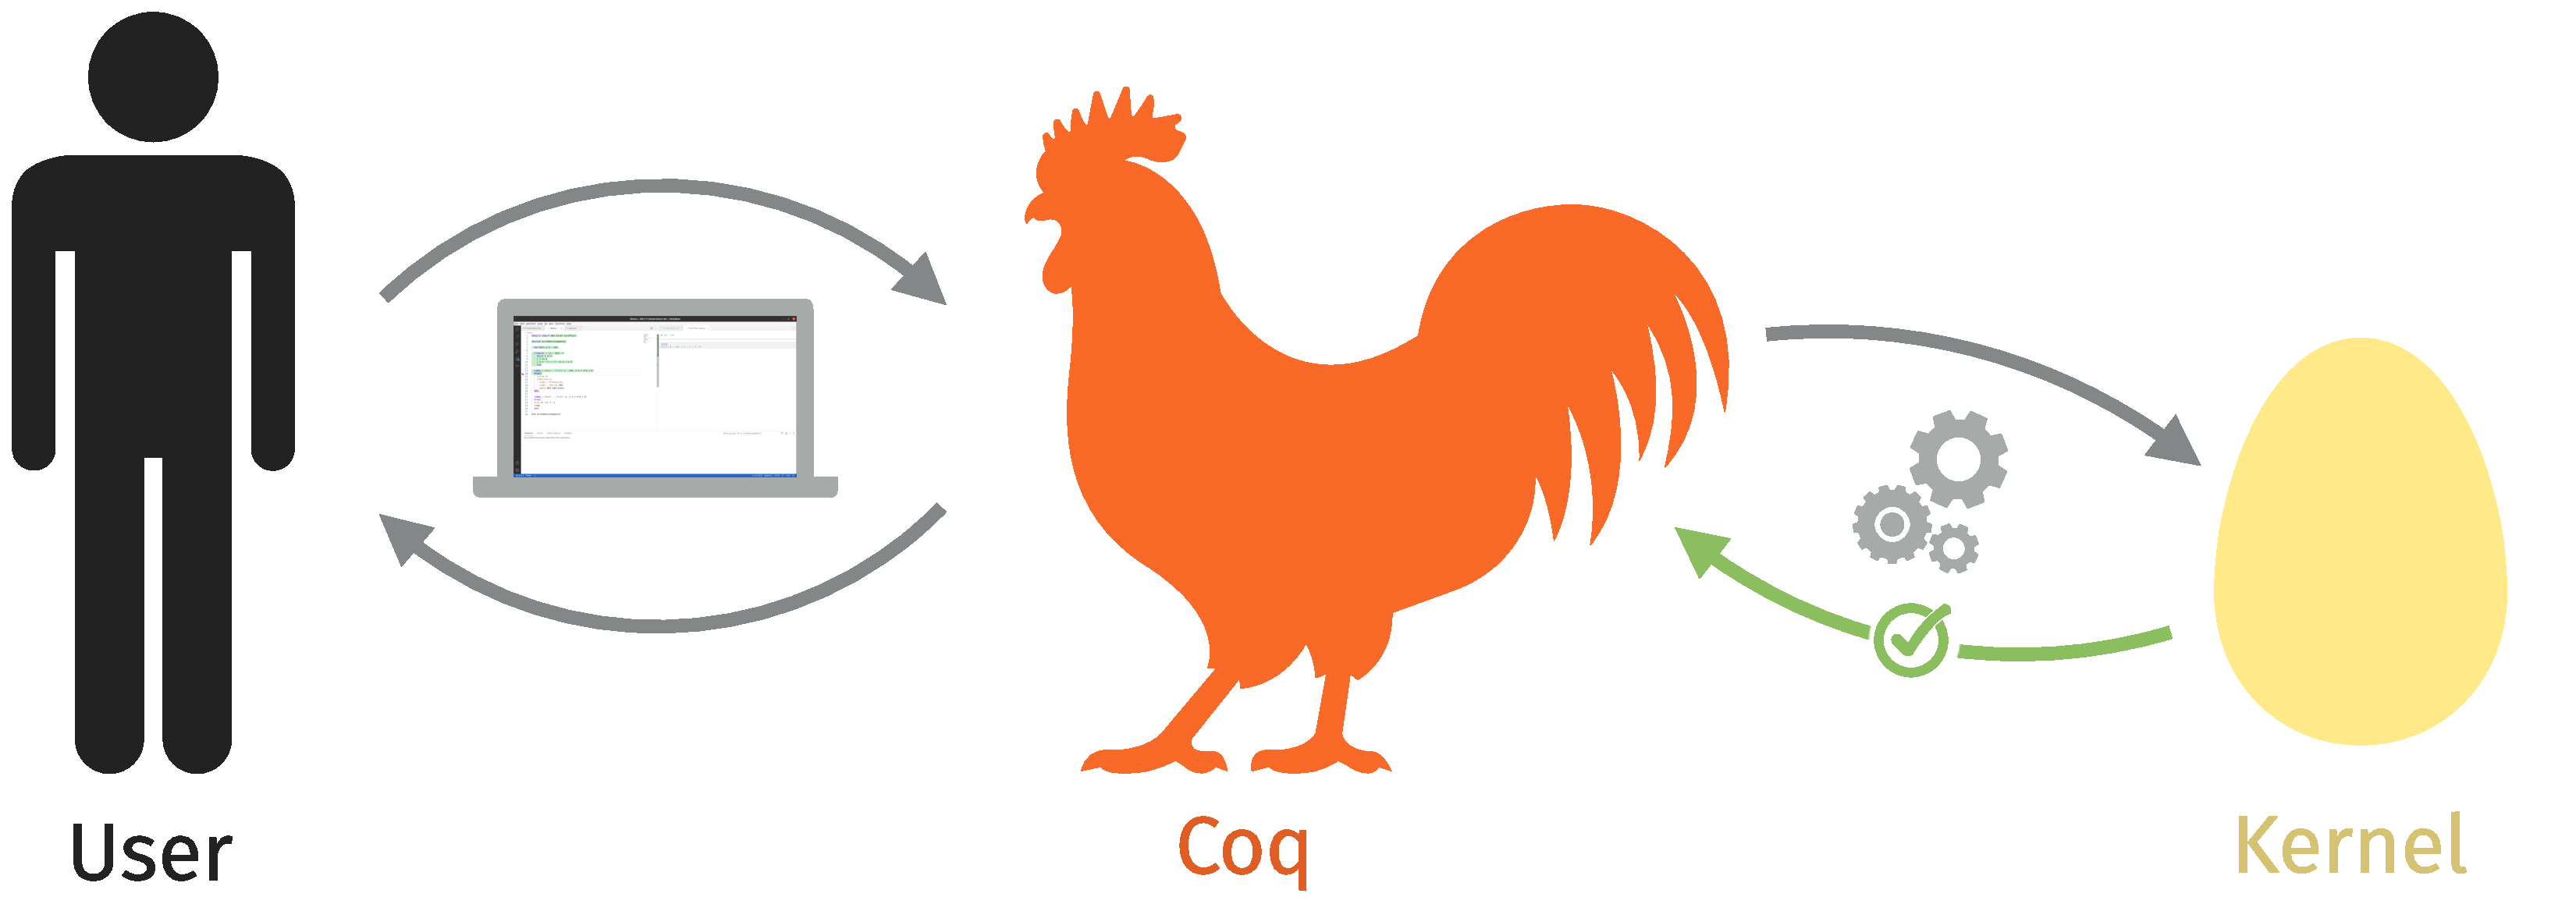
\includegraphics{./figures/coq-kernel-en.pdf}

  \caption{\kl{Coq}’s schematic architecture}
  \label{fig:coq-en}
\end{figure}

\kl{Coq} is based upon the \kl{Curry-Howard correspondence}: proofs are seen as programs,
in a language called \intro{Gallina}, and their verification is done using an algorithm
close to those used for types in conventional languages. However, if, in the first versions
from the 80s, \kl{Coq} looked like a somewhat esoteric programming language, it is
currently not at all the case anymore. The reason is that the major part of the tool in its
current versions aims at helping the user in generating a correct proof. It is a true
\kl[proof assistant]{proof \emph{assistant}}!
The way \kl{Coq} works is illustrated in \cref{fig:coq-en} : the user interactively exchanges
with \kl{Coq}, which uses this interaction to generate a proof term. This proof term is then
sent to a very specific part of the tool, called the \intro{kernel}.
This is the part implementing the type-checking algorithm, and thus responsible for ensuring
that the proof terms built interactively are correct.
The \kl{kernel} is thus the crucial part of the \kl{Coq}, because it is the one – and only –
ultimately responsible for proof-checking.

This architecture, which clearly isolates the critical part of the system, is called
\intro{De Bruijn criterion} \sidecite{Barendregt2001}, in tribute to one of the pioneer
of proof assistants.
If the rest of the ecosystem has grown much more than the \kl{kernel} since the beginning,
the latter has also evolved, becoming gradually more complex.
And, as any other software development, it is not out of bugs%
\sidenote{ The magnitude is that of one critical bug found every year, a list is maintained
at the following address: \url{https://github.com/coq/coq/blob/master/dev/doc/critical-bugs}}.
These are in general hard to exploit by a user, even more so without noticing.
But still, they exist, and since the \kl{kernel} tends to get more and more complex, they
are likely to continue appearing.

\subsection{\kl{MetaCoq}, a formalization in \kl{Coq}, for \kl{Coq}}[\kl{MetaCoq}]

If we wish to guarantee a trust level as high as possible in the \kl{kernel}, we must
resort to new ideas. The \kl{MetaCoq} project aims at answering this problematic. The idea
is simple: using \kl{Coq} itself to certify the correctness of its \kl{kernel}.

More precisely, the first step is to describe formally the type system on which the \kl{kernel}
is based, and to show its theoretical properties.
Once these are established, the second step
% \sidenote{This is the one on which I mostly work, and on which we will come back in more
% length later on.}
consists in implementing a type-checking algorithm as close as possible to the one of the
\kl{kernel}, directly in \kl{Gallina}%
\sidenote{Indeed, thanks to the \kl{Curry-Horward correspondence}, \kl{Gallina} is of
course a proof language, but also a true programming language!}.
We show while defining the algorithm that it is indeed \reintro(bidir){correct}%
\sidenote{If the algorithm pretends that a term is well-typed, then it is the case.}
and \reintro(bidir){complete}%
\sidenote{The algorithm answers positively on all well-typed programs.}
Finally, in a third step, we extract out of this certified \kl{Gallina} program another,
more efficient program, by erasing the content related to the proof of correctness, in order
to keep only the algorithmically relevant one.
This extraction is a complex step, but crucial if we wish to replace the current \kl{kernel}
while keeping a reasonable efficiency. Therefore, once again we prove that said extraction
is correct%
\sidenote{Meaning that it preserves the semantics of programs.},
once again by programming it in \kl{Gallina}.

\subsection{Checking, inference and bidirectional typing}[Bidirectional typing]

During the second phase, in order to prove that the algorithm is complete, it is
very useful to go through an intermediate specification, more structured than the
theoretical specification of the first phase.
In particular, it is important to separate two close questions, but very distinct:
one one side, type-checking, where we try and \emph{check} that a term indeed has a
given type;
on the other side, inference, where we try and \emph{find} a type for a term, if such a
type exists.
The typing algorithm of \kl{Coq}'s \kl{kernel} is \intro{bidirectional}, that is it
alternates all the time between these two notions when it checks that a term is well-typed.
This bidirectional structure being closer to the algorithm, describing it formally allows to
clearly separate between, on one side, its equivalence with the original formalization, and
on the other, the part purely dedicated to implementation questions.

In the specific case of dependent types, even if present in type-checking algorithms since
the origin – see \eg \sidecite{Huet1989} –, bidirectional typing has been relatively little
studied. However, beyond its strong relation to algorithms, this approach also presents
theoretical advantages: thanks to its more constrained structure than the standard presentation,
to obtain properties difficult to obtain in that context.

\subsection{Gradual types: some flexibility in a desperately static world}
  [Types graduels]
\label{sec:intro-graduel-en}

There are two main approaches to program type-checking. In the static approach%
\sidenote{On which \kl{Coq} is based.}
types are verified prior to the execution, whereas, in the dynamic approach, the well-typedness
of the operations is verified on the fly during that same execution.
The dynamic discipline is more flexible, as it enable us to verify exactly what is necessary
for the good execution of a program.
The strictness of static typing, conversely, allows for error detection earlier in the
development, and imposes invariants useful in order to optimise compilation or execution.
Instead of opting exclusively for one of the two approaches, \intro{gradual typing}
\sidecite{Siek2015} aims at integrating the static and dynamic disciplines in one and the
same language. This gives access to a whole specter of options, from a rigid completely static
discipline to a flexible dynamic one, in particular allowing for a fine-grained, local choice
of how each part of a program is type-checked.
In particular, one can evolve the discipline during software development, benefiting from
the flexibility of dynamic typing in early phases, and from the guarantees of static typing
later on.

As the case of \kl{MetaCoq} illustrates, \kl{Coq} can be used as a true programming language.
Even better: its type system can express very complex properties of programs, and thus
verify even before their execution that the code indeed enforces them.
Sadly, this impossibility to write imperfect code can turn against the user, by making the
early development phase more difficult. Indeed, nobody writes correct code on the first try,
and it would often be nice to temporarily lift the strong guarantees of typing in order to
facilitate experimentation The idea would then be to take inspiration from gradual typing,
in order to permit a more flexible logical or software development. Once again,
\kl{Curry-Horward correspondence} is at work, since we adapt concepts from the world of
programming languages to the logical one.

\section{And this thesis?}
\label{sec:this-thesis}

My doctoral work itself is centered around bidirectional typing, under three main aspects,
corresponding to the three parts of this thesis.
They are preceded by \cref{chap:tech-intro}, which introduces the main technical notions
used in what follows.

\subsection{Theory of bidirectional typing}

The first part (\nameref{part:bidir}) proposes to fill a part of the theoretical gap around
bidirectional typing for dependent types. It in particular contains a proof of equivalence
between the standard presentation of the literature, and a bidirectional one.
\Cref{chap:bidir-ccw} presents the general ideas that guide this work in a relatively
simple setting, in order to ease the exposition. \Cref{chap:bidir-pcuic} shows how to extend
them to a more realistic setting, close to the type theory implemented in \kl{Coq}.
Finally, \cref{chap:bidir-conv} focuses on the particular status of conversion%
\sidenote{This crucial notion allows the integration into dependent type theory of
the notion of computation of programs.},
and the links between recent work on this subject and bidirectional typing.

\subsection{Bidirectional typing in \kl{MetaCoq}}

The second part of the thesis (\nameref{part:metacoq}) focuses on the \kl{MetaCoq} project,
and in particular the formalization, in \kl{Coq}, of the ideas presented in the first part.
\Cref{chap:metacoq-general} gives a general overview of the project, while
\cref{chap:kernel-correctness} concentrates more specifically on the proof that the
\kl{kernel} implemented in \kl{MetaCoq} fulfils its specification.

\subsection{Gradual dependent types}

Finally, the third and last part (\nameref{part:gradual}) presents my work in the area
of \kl{gradual types}. Since dependent types already form complex systems, their adaptation
to the gradual approach is particularly delicate. A summary of the possibilities issues is
presented in \cref{chap:gradual-dependent}. An interesting point to emphasise is that the
usual presentation of dependent types turns out to be unsuited, because too flexible.
The additional structure provided by bidirectional typing is thus important. It also
appeared as relevant to present the type-directed elaboration of terms from a source language
to a target one, an important characteristic shared by all \kl[gradual]{gradual languages}.
The use of a bidirectional elaboration, and the properties it allows to obtain, are described
in \cref{chap:bidir-gradual-elab}. Finally, \cref{chap:beyond-gcic} succintly describes the
rest of the work I took part in in the context of gradual types, but which is not directly
linked to bidirectional typing.

\subsection{Technical contributions}

My doctoral work started with the study of \kl{gradual} \kl(typ){dependent} types.
I contributed, together with Kenji Maillard, Nicolas Tabareau and Éric Tanter, to
\sidetextcite{LennonBertrand2022}, where we study a gradual extension to the
Calculus of Inductive Constructions. My main technical contribution corresponds
to \cref{chap:bidir-gradual-elab}. \Cref{chap:gradual-dependent} also comes from this
publication. A second article, together with the same authors and in the continuity of the
previous one, is currently under peer-reviewing. It is quickly summarized in
\cref{chap:beyond-gcic}, together with the second technical part of
\textcite{LennonBertrand2022}, whose main contributor is Kenji Maillard.

This work having shown the interest of a bidirectional dependent type system and the relative
scarceness of results on the subject, I turned to a more detailed study of it, both on
paper and by means of a formalization based on \kl{MetaCoq}. This led to a second publication
\sidecite{LennonBertrand2021}, and corresponds to \cref{chap:bidir-ccw,chap:bidir-pcuic},
and parts of \cref{chap:kernel-correctness}.

I then worked to the integration of this formalization into \kl{MetaCoq}, and its use
in order to prove completeness of the \kl{kernel} it implements. This corresponds to the
rest of \cref{chap:kernel-correctness}. I also took part into the project on more minor points.
This part of my thesis work has not been published yet, but the other contributors to
\kl{MetaCoq} and I are currently working on it.

Finally, \cref{chap:bidir-conv} corresponds to a project I started in order to extend
\kl{MetaCoq}, but which did not reach the stage of publication yet.